\chapter{Web platform}
\label{cap3}

This chapter details the design, development, and testing of the interactive web platform created for this project. The platform serves as the primary user-facing interface, enabling seamless protein sequence analysis, functional annotation via external deep learning APIs, and 2D structure visualization through locally implemented optimization algorithms. The chapter outlines the system requirements, describes the interface prototype, explains the technical implementation and architecture, and discusses the testing procedures employed to ensure reliability and correctness.

% ─────────────────────────────────────────────────────────────────────
\section{Requirement analysis}
\label{cap3:sec_requirements}

To provide a robust and accessible tool for computational biology, the web platform was designed to meet the following functional and non-functional requirements:

\begin{itemize}
    \item \textbf{Sequence Input Processing:} The system must accept protein sequences in standard FASTA format, capable of parsing multiple sequences simultaneously. A dedicated utility function strips FASTA headers (lines beginning with \texttt{>}) and validates that only legal amino acid characters are processed.

    \item \textbf{Function Prediction Integration:} The platform must seamlessly integrate with the external \textbf{DeepGO} API~\cite{kulmanov2018deepgo} to retrieve and display Gene Ontology (GO) terms categorized into three domains: Biological Process (GO:BP), Molecular Function (GO:MF), and Cellular Component (GO:CC).

    \item \textbf{Algorithm Selection and Configuration:} Users must be able to select from a suite of 2D structure prediction algorithms Hill Climbing (HC), Simulated Annealing (SA), Monte Carlo (MC), Replica Exchange Monte Carlo (REMC), and the trained Deep Q-Network (DQN) and configure their respective hyperparameters (e.g., number of iterations, temperature range, number of replicas, number of DQN rollouts, and visualization step interval). The final interface configuration is illustrated in Appendix~A.

    \item \textbf{Structure Visualization:} The platform must generate a visual SVG-based representation of the folded protein on a 2D HP lattice, accurately depicting Hydrophobic (H) and Polar (P) amino acids with distinct colors, rendering the backbone chain, and reporting the total computed energy.

    \item \textbf{3D Structure Retrieval:} As an extended feature, the system should act as a bridge to fetch known or predicted 3D structures from the \textbf{AlphaFold DB}~\cite{varadi2022alphafold} and the \textbf{ESMFold API}~\cite{lin2023evolutionary}, returning PDB-format files for further visualization.

    \item \textbf{Responsiveness and Usability:} The interface must be responsive across different screen sizes and provide clear, user-friendly error messages for invalid inputs, API failures, or algorithm errors.
\end{itemize}

% ─────────────────────────────────────────────────────────────────────
\section{User prototype}
\label{cap3:sec_prototype}

The user interface was prototyped with a focus on simplicity, clarity, and ease of use for researchers and students unfamiliar with command-line tools. The layout is divided into the following sections:

\begin{itemize}
    \item \textbf{Input Interface:} A prominent text area allows users to paste raw FASTA sequences. A set of radio buttons and dropdown menus positioned below the input box allow the user to select the desired action (\textit{Predict GO Terms} or \textit{Generate 2D Structure}) and choose a specific optimization algorithm.

    \item \textbf{Hyperparameter Panel:} When the \textit{Structure} action is selected, context-sensitive input fields appear dynamically, allowing experienced users to fine-tune algorithm parameters. For example: number of iterations for HC/SA/MC, number of replicas and temperature range for REMC, number of DQN rollouts, and the interval at which intermediate folding steps should be displayed.

    \item \textbf{Results Dashboard:} The output is presented in a structured panel. For function prediction, GO terms are displayed in categorized, expandable lists with their associated confidence scores. For structure prediction, the interface renders the 2D lattice graphically using an auto-scaling SVG canvas, highlighting H residues (colored) and P residues (distinct color), drawing the backbone chain, and displaying the computed minimum energy. A step explorer allows users to inspect intermediate conformations every user-defined number of iterations; for DQN, this corresponds to the constructive residue-by-residue folding trajectory. Appendix~B shows representative screenshots of this step-by-step visualization from the initial partial chain to the final conformation.

    \item \textbf{3D Viewer Integration:} A dedicated section allows users to enter a UniProt accession code and fetch the corresponding 3D structure from AlphaFold DB or ESMFold, displaying or providing a download link to the resulting PDB file.
\end{itemize}

% ─────────────────────────────────────────────────────────────────────
\section{Implementation}
\label{cap3:sec_implementation}

The web platform was implemented using \textbf{Django 6.0.2}, a high-level Python web framework that encourages rapid development and clean, pragmatic design~\cite{django2024}. The overall system follows a \textbf{Model-View-Template (MVT)} architecture.

\begin{figure}[htbp]
\centering
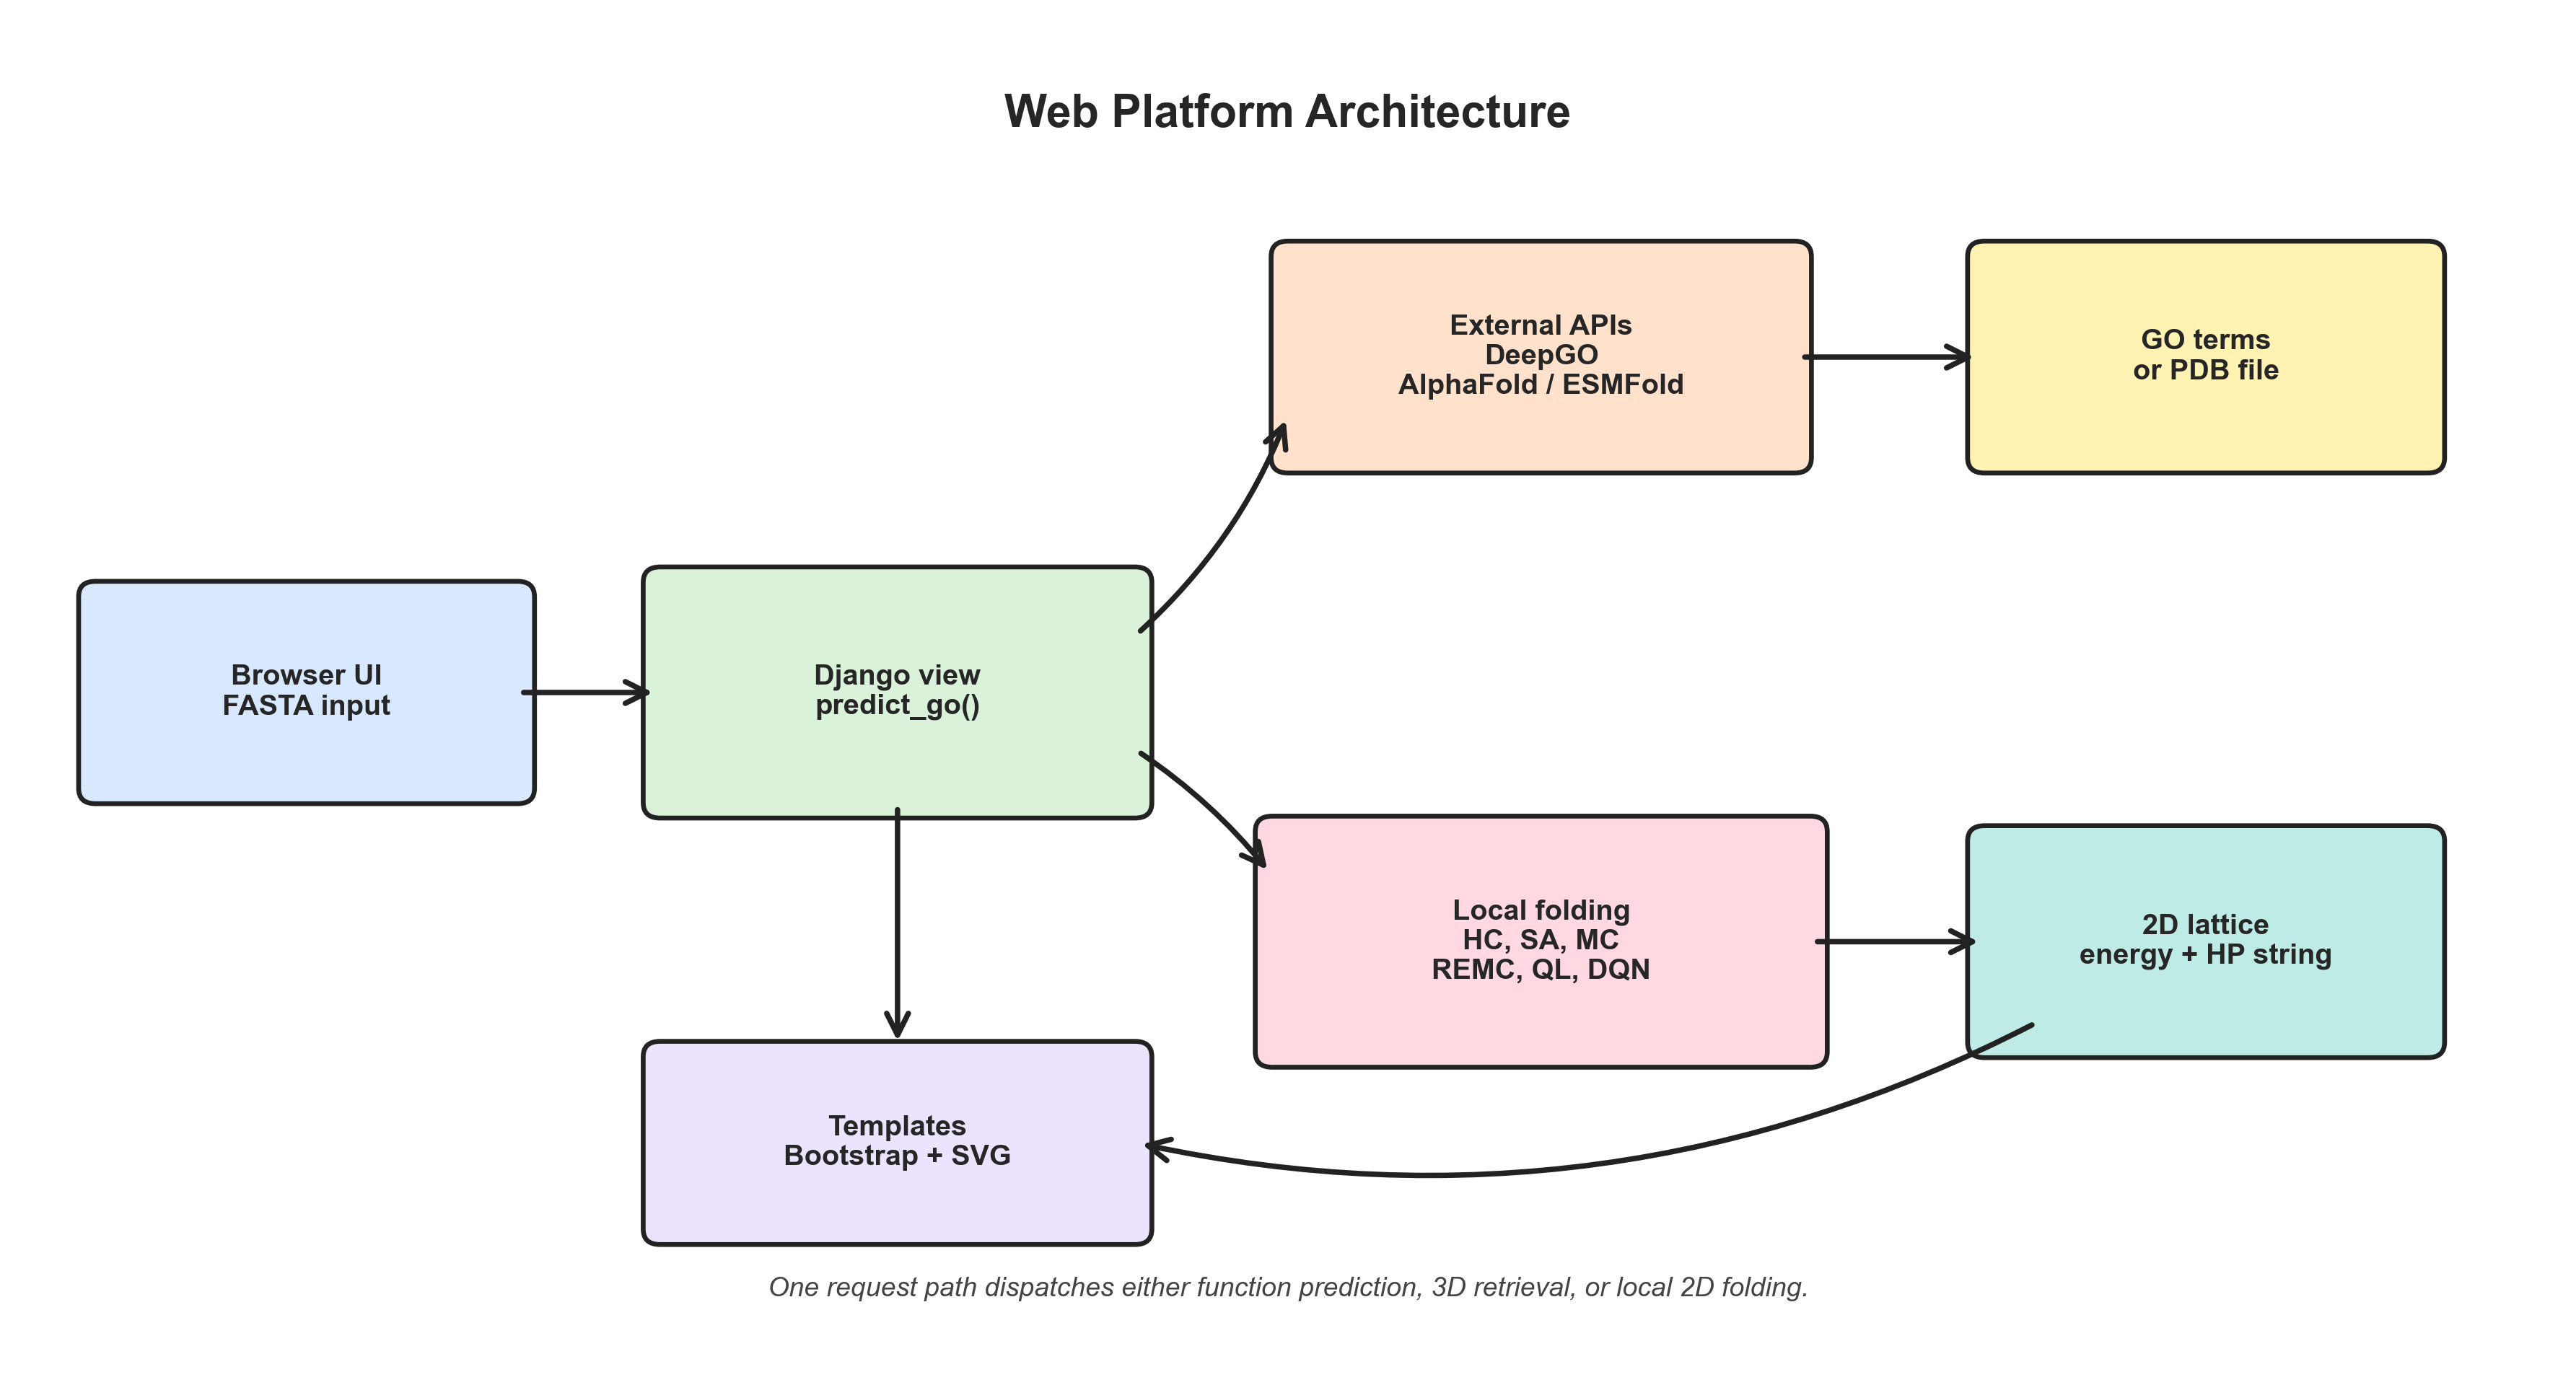
\includegraphics[width=\textwidth]{Figuras/web_platform_architecture.png}
\caption[Web platform architecture]{High-level architecture of the web platform. A single Django view dispatches requests to either external services for function/3D prediction or local HP-folding algorithms for 2D structure generation.}
\label{fig:web_platform_architecture}
\end{figure}

\subsection{Backend architecture}
\label{cap3:subsec_backend}

The core logic resides in \texttt{go\_predictor/views.py}, which acts as the controller:

\begin{itemize}
    \item \textbf{Request routing:} The main view function receives \texttt{POST} requests containing the FASTA sequence, the selected action, and hyperparameter values. It dispatches processing to the appropriate function based on the action type.
    \item \textbf{FASTA parsing:} A utility function strips header lines and concatenates residue characters, performing basic validation (only A--Z characters representing amino acids are accepted).
    \item \textbf{HP translation:} The raw amino acid sequence is converted to a binary HP string using a fixed hydrophobic residue set (\texttt{ACFILMVWY}), following the standard HP model classification.
\end{itemize}

\subsection{Algorithmic integration}
\label{cap3:subsec_algo_integration}

The web application dynamically imports the production structure prediction scripts located in the project's \texttt{tests/} directory and the trained DQN inference module. This modular architecture decouples the web interface from the computational logic:

\begin{itemize}
    \item \texttt{test\_hc.py} --- Hill Climbing (\texttt{generate\_2d\_structure})
    \item \texttt{test\_sa.py} --- Simulated Annealing (\texttt{generate\_2d\_structure\_sa})
    \item \texttt{test\_mc.py} --- Monte Carlo (\texttt{generate\_2d\_structure\_mc})
    \item \texttt{test\_remc.py} --- Replica Exchange Monte Carlo (\texttt{generate\_2d\_structure\_remc})
    \item \texttt{agent\_dqn\_model.py} --- Constructive DQN inference (\texttt{run\_dqn\_inference})
\end{itemize}

Each function returns a list of $(x, y)$ lattice coordinates and the best energy found. For interactive visualization, the classical algorithms can optionally return trace frames at a user-defined interval, while the constructive DQN returns residue-placement frames. The view passes these coordinates to the SVG renderer, which maps them to pixel positions on an auto-scaling canvas. The Tabular Q-Learning implementation remains available in \texttt{test\_ql.py} for offline benchmarking, but it is not imported by the production web view because the trained DQN replaces it for real-time inference.

\subsection{External API communication}
\label{cap3:subsec_api}

The \texttt{requests} library is used to communicate with external services:

\begin{itemize}
    \item \textbf{DeepGO API:} The \texttt{call\_deepgo\_api} function packages the user's sequence into a JSON payload and sends a \texttt{POST} request to the DeepGO inference endpoint. The returned JSON containing GO term identifiers and confidence scores for all three ontology domains is parsed and structured for display in the template.
    \item \textbf{AlphaFold DB:} A \texttt{GET} request is sent to the AlphaFold prediction API using the UniProt accession as query input. This retrieves the metadata associated with the specified protein. The application then extracts the \texttt{pdbUrl} field returned by the API and uses it to download or render the corresponding PDB file. This avoids hard-coding a specific AlphaFold file-version suffix such as \texttt{model\_v4}.
    \item \textbf{ESMFold API:} A \texttt{POST} request to the ESMFold endpoint sends the raw sequence and receives a PDB-format response, allowing users to obtain predicted structures without a local installation.
\end{itemize}

All external calls are wrapped in \texttt{try-except} blocks to handle network timeouts, invalid accession codes, and API rate limits, returning descriptive error messages to the user rather than server faults.

\subsection{Frontend design}
\label{cap3:subsec_frontend}

The frontend is built with \textbf{HTML5}, \textbf{CSS3}, \textbf{Tailwind CSS}, and Lucide icons to ensure a responsive and visually consistent layout. Django's template engine is used to dynamically inject algorithmic results, loop over GO term lists, and conditionally show/hide interface sections based on the selected action. The SVG 2D structure visualization is embedded directly into the response HTML and updated client-side by JavaScript when the user moves the step slider.

% ─────────────────────────────────────────────────────────────────────
\section{Tests}
\label{cap3:sec_tests}

Rigorous testing was conducted to ensure the platform's stability, accuracy, and robustness:

\begin{itemize}
    \item \textbf{Integration Testing:} The Django backend was verified to correctly invoke the standalone algorithmic scripts with the parameters provided by the user interface. Edge cases were tested: sequences of length 1 (single residue), sequences composed entirely of 'P' residues (zero H-H contacts, energy $= 0$), and very long sequences ($> 100$ residues) to verify graceful degradation.

    \item \textbf{FASTA Validation:} The parser was tested against malformed inputs missing headers, sequences with non-amino-acid characters, empty submissions, and mixed-case inputs confirming that invalid data is rejected with user-friendly error messages before reaching the computational modules.

    \item \textbf{API Reliability:} Connections to DeepGO, AlphaFold, and ESMFold were tested under simulated failure conditions (invalid accession codes, network unavailability). Exception handling confirmed that the server returns descriptive error messages rather than \texttt{500 Internal Server Error} responses.

    \item \textbf{Visualization Correctness:} The SVG renderer was validated by comparing the rendered structures against manually computed expected positions for small sequences (up to 10 residues), verifying that backbone links connect consecutive residues and that H/P color assignments are consistent with the HP string.

    \item \textbf{Hyperparameter Passthrough:} It was verified that user-specified hyperparameter values (e.g., \texttt{iterations=50000}, temperature values, replica counts, DQN rollouts, and step-visualization intervals) are correctly parsed from the form POST data, validated to be in acceptable ranges, and passed to the underlying algorithm functions.
\end{itemize}

% ─────────────────────────────────────────────────────────────────────
\section{Summary}
\label{cap3:sec_summary}

This chapter described the design and implementation of the web platform that serves as the user-facing component of the project. The requirement analysis guided the development of a functional interface prototype, which was implemented using Django's MVT architecture, cleanly separating web request handling from the computationally intensive algorithmic logic. The modular algorithmic integration allows the implemented algorithms (HC, SA, MC, REMC and DQN) to be invoked through a unified interface. External API communication with DeepGO, AlphaFold, and ESMFold was robustly handled with appropriate error management. Comprehensive testing confirmed that the platform correctly handles user inputs, algorithm execution, step visualization, and external API interactions across a range of normal and edge-case scenarios.
